\begin{frame}
  \titlepage
  \begin{figure}[ht]
      \begin{center}
          
\includegraphics[height=1in]{images/logo-taller.png}
      \end{center}
  \end{figure}
\end{frame}

\begin{frame}{Motivación 1/2}

    \begin{figure}[ht]
        \begin{center}
            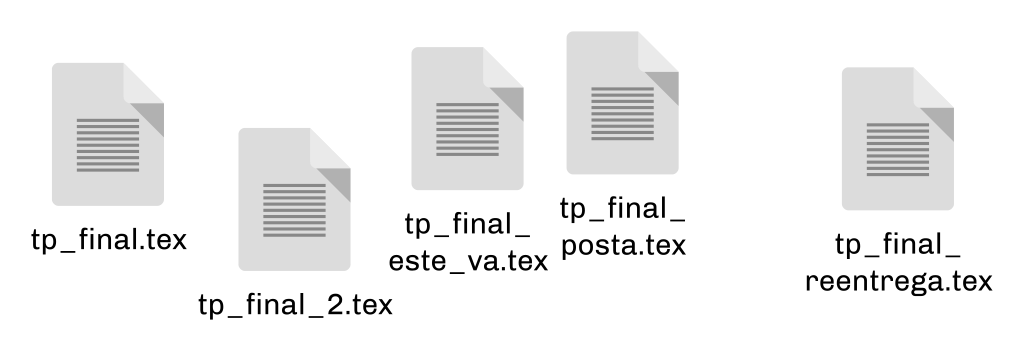
\includegraphics[height=1.5in]{images/caos.png}
        \end{center}
    \end{figure}

    \pause
    \begin{figure}[ht]
        \begin{center}
            
\includegraphics[height=1.5in]{images/horror.png}
        \end{center}
    \end{figure}

\end{frame}

\begin{frame}{Motivación 2/2}

    \begin{block}{Trabajando de a grupo}
        \begin{itemize}
            \item Enviar cambios por mail, o
            \pause
            \item Sincronizar cambios por Dropbox, o
            \pause
            \item Sincronizar cambios por Google Docs.
        \end{itemize}
    \end{block}

    \pause
    \begin{figure}[h]
        \begin{center}
            
\includegraphics[height=1.5in]{images/horror.png}
        \end{center}
    \end{figure}

\end{frame}

\begin{frame}{¿Qué es un Sistema de Control de Versiones?}

	\begin{block}{}
		Los Sistemas de Control de Versiones son una categoría de programas que permiten a un equipo manejar los cambios en el código fuente de un proyecto a lo largo del tiempo.

		Dichos programas llevan un seguimiento de las modificaciones que hacemos al código, y en caso de que nos equivoquemos en algo es posible volver a tras y comparar el código actual con otras versiones anteriores para ayudar a arreglar el error.

		También, permiten que varias personas distintas del equipo modifiquen el código a la vez y compartan los cambios, tratando que prevenir posibles conflictos, y en caso de que los hubiera ayudando a identificarlos y resolverlos.

	\end{block}

    \pause
    \begin{resumen}{Es decir..}
        \begin{itemize}
            \item Permiten arreglar \textit{accidentes} y volver a versiones anteriores del código.
            \item Permiten compartir código con otras personas.
        \end{itemize}
	\end{resumen}

\end{frame}

\begin{frame}{¿Qué es Git?}

	\begin{block}{}
		Git es un Sistema de Control de Versiones \textbf{distribuido y de código abierto}.
        Además fue diseñado con enfasis en la \textbf{performance} (para manejar proyectos muy grandes), \textbf{seguridad} y \textbf{flexibilidad}.
        Provee un amplio conjunto de comandos que permiten realizar operaciones de alto y bajo nivel.
	\end{block}

    \begin{figure}[ht]
        \begin{center}
            
\includegraphics[height=1.5in]{images/logo-git.png}
        \end{center}
    \end{figure}
\end{frame}

\begin{frame}[fragile]{Configuraciones iniciales}

	\begin{block}{Clave ssh}
		Para poder trabajar comodamente con repositorios Git que estén en internet (GitHub, Bitbucket, GitLab, etc) podemos configurar una clave ssh que nos identifique con el servidor que estemos usando.

        Por ejemplo, en GitLab:

        \url{http://doc.gitlab.com/ce/gitlab-basics/create-your-ssh-keys.html}
	\end{block}

    \begin{block}{Tu identidad}
        Es importante establecer nuestro nombre y email ya que estos van a ir asociados con los cambios que hagamos:

        \vspace{0.5em}

        \texttt{git config --global user.name "John Doe"}

        \texttt{git config --global user.email johndoe@example.com}
    \end{block}


\end{frame}

\begin{frame}[t]{Obteniendo un repositorio Git}
%    \begin{block}{Inicializando un repositorio en un directorio existente}
%        Para crear un nuevo repositorio local podemos ir al directorio y ejecutar
%        \texttt{git init}. Esto crea un subdirectorio \textit{.git} que tiene todos
%        los archivos necesarios del repositorio.
%    \end{block}

%    \begin{block}{Clonando un repositorio existente}
    \begin{comando}
        git clone
    \end{comando}

    \pause
	\begin{block}{}
        Para obtener una copia local de un repositorio existente en algún servidor,
        utilizamos el comando \texttt{git clone [URL]} (sin los corchetes)
    \end{block}

    \pause
    \vspace{1em}
    \begin{ejercicio}{Ejercicio}
        \textit{Clonar} el repositorio que tiene URL: \textbf{git@gitlab.com:talleres-comcom/taller-git.git}

        \vspace{0.5em}
        Es un repositorio que tiene los fuentes\ \LaTeX\ de estas diapositivas !
    \end{ejercicio}
\end{frame}

\begin{frame}[t]{Preparando cambios}

    \begin{comando}
        git add
    \end{comando}

    \pause
    \begin{block}{}
        \begin{enumerate}
            \item Creamos/Modificamos el archivo en cuestión.
            \item Ejecutamos \texttt{git add [nombre del archivo]}
        \end{enumerate}
    \end{block}

    \pause
    \vspace{1em}
    \begin{ejercicio}{Ejercicio}
        Adentro del repositorio que \textit{clonaron} recién, crear un archivo y
        marcarlo como \textit{preparado} usando el comando \texttt{git add}.
    \end{ejercicio}

\end{frame}

\begin{frame}[t]{Confirmando cambios}

    \begin{comando}
        git commit
    \end{comando}

    \pause
    \begin{block}{}
        Una vez que tenemos \textit{preparados} los cambios a confirmar,
        ejecutamos\\ \texttt{git commit -m [mensaje]}.

        Dónde [mensaje] índica al que lea eso cuales fueron los cambios que acabamos de confirmar.
    \end{block}

    \pause
    \vspace{1em}
    \begin{ejercicio}{Ejercicio}
        Confirmar los cambios que \textit{prepararon} en la diapo anterior.
    \end{ejercicio}

\end{frame}

\begin{frame}[fragile, t]{¿Está preparado, confirmado o ninguna de las dos?}

    \begin{comando}
        git status
    \end{comando}

    \begin{block}{No es lo mismo!}
        Las modificaciones que hacemos pueden estar en \textbf{3 estados} distintos:
        \begin{itemize}
            \pause
            \item<2-> \textbf{Modificado (modified)}: las modificaciones todavía no están \textit{preparadas o listas}.
            \item<3-> \textbf{Preparado (staged)}: las modificaciones están marcadas como \textit{preparadas o listas} e
                irán en la proxima \textit{confirmación de cambios}.
            \item<4-> \textbf{Confirmado (committed)}: las modifiaciones están guardadas con un \textit{mensaje} que explica los cambios realizados.
        \end{itemize}
    \end{block}

    \only<2> {
        \gitstatusmodified
    }
    \only<3> {
        \gitstatusready
    }
    \only<4> {
        \gitstatusclean
    }

\end{frame}

\begin{frame}{Colaborando con otras personas}

    Los repositorios remotos son \textit{copias} de tu proyecto a las cuales accedemos a través
    de Internet. Puede haber varios, cada uno de los cuales
    puede ser de sólo lectura, o de lectura/escritura, según los permisos que tengamos.

    \vspace{0.5em}

    Colaborar con otros implica gestionar estos repositorios remotos, y mandar (\textbf{push}) y recibir (\textbf{pull})
    datos de ellos cuando necesites compartir cosas.

\end{frame}

\begin{frame}[t]{Enviando cambios}
    \begin{comando}
        git push
    \end{comando}

    \begin{block}{}
        \begin{itemize}
            \item
            \item
            \item
        \end{itemize}
    \end{block}
\end{frame}

\begin{frame}[t]{Trayendo cambios}
    \begin{comando}
        git pull
    \end{comando}
\end{frame}

\begin{frame}[t]{Y qué pasa sí.. BOOM}
    A veces hay conflictos.

\end{frame}

\begin{frame}[t]{Creando un repositorio vacio}
    \begin{comando}
        git init
    \end{comando}
\end{frame}

\begin{frame}[t]{Añadiendo un repositorio remoto}
    \begin{comando}
        git remote
    \end{comando}

    % Para ver qué repositorios remotos están configurados, podemos usar el comando \texttt{git remote}.
    % Si acabamos de clonar el repositorio que tiene los fuentes de estas diapositivas y corremos \texttt{git remote -v}, veremos:
    % \begin{verbatim}
    % origin  git@github.com:FlyingPumba/git-intro.git (fetch)
    % origin  git@github.com:FlyingPumba/git-intro.git (push)
    % \end{verbatim}
    %
    % Y si tenemos un repositorio creado localmente y queremos añadir un remoto, usamos \texttt{git remote add [nombre] [url]}.
\end{frame}

\begin{frame}[t]{A practicar !}
    Ejercicio largo de conflictos y GitLab.

\end{frame}
